% !TEX root =  master.tex
\chapter{Analyse} \label{analyse}
	
%	\section{Anforderungsanalyse}
	
	\section[Ist-Analyse]{Ist-Analyse {\hfill \normalsize Yvonne Werner}}\label{istAnalyse}
	Mithilfe der Ist-Analyse wird eine bestehende Lösung zur Reservierung von Kinokarten betrachtet. Diese bildet die Grundlage für die Evaluierung eines möglichen Aufbaus von Kinoreservierungssystemen. Dabei spielen vor allem die Verständlichkeit der Seite und die verschiedenen Reservierungsschritte eine entscheidende Rolle. Zu letzterem wird betrachtet, welche Aktionen der Nutzer durchlaufen kann bzw. muss um eine Reservierung vorzunehmen und auf welche Seiten er dabei weitergeleitet wird.Dadurch wird versucht herauszufinden, welche Funktionen für eine Reservierung essenziell sind und welche Schritte zusätzliche Funktionen darstellen. Des Weiteren wird darauf geachtet, wie eine Reservierung erfolgen kann, d.h. ob die Notwendigkeit eines Benutzerkontos zwingend besteht oder ob eine Reservierung ebenfalls als Gast möglich ist. 
	
	\subsection{Kinopolis Viernheim}
	Im Folgenden wird die Internetseite des Kinopolis in Viernheim\footnote{https://www.kinopolis.de/vi} als Vorlage zur Evaluierung eines Kinoreservierungssystems verwendet. 
	
	\subsubsection{Startseite}
	Beim Öffnen der Startseite von Kinopolis Viernheim fällt direkt auf, dass die eigentliche Hauptseite des Kinos von einem Rahmen mit Werbung für einen aktuellen Film umgeben ist (siehe Abb. \vref{fig:Kinop.Start}). Dadurch erscheint die eigentliche Seite als ziemlich klein und rückt in den Hintergrund. Allerdings kann das Kino auf diese Weise Werbung für aktuelle Filme machen und der Kunde kann durch das Anklicken des Rahmens  auf die Übersichtsseite des Films weitergeleitet werden. 
	\begin{figure}[H]
		\centering 
		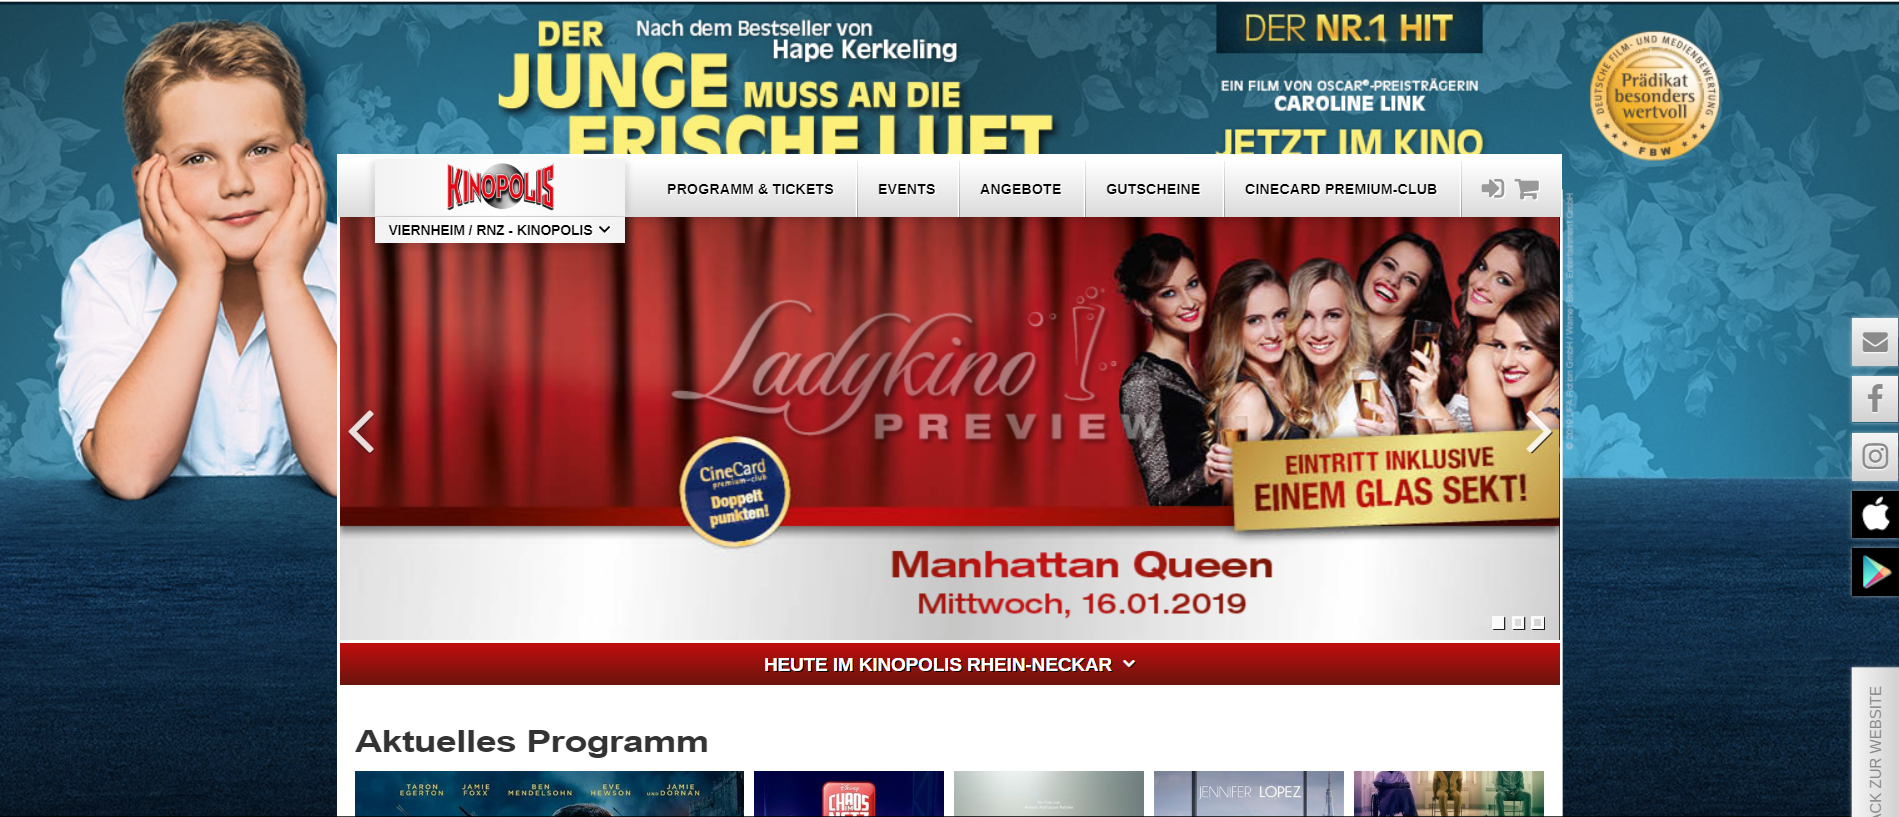
\includegraphics[width=14cm]{img/Kinopolis_MA_Startseite.png}
		\captionsetup{format=hang}
		\centering\caption[Startseite von Kinopolis Viernheim]{\label{fig:Kinop.Start}Startseite \\Quelle: Kinopolis Viernheim}
	\end{figure} 
	
	Die eigentliche Hauptseite in der Mitte enthält ganz oben eine Kopfleiste, in der zwischen Programm \& Tickets, Events, Angeboten und Gutscheinen gewählt werden kann. Außerdem besteht für den Kunden die Möglichkeit eine Premium-Club Card zu erstellen. Dadurch wird es ihm ermöglicht Punkte zu sammeln, die der Eigentümer der Karte in Vorteile umwandeln kann. Des Weiteren ist über ein Symbol die Anmeldung zu einem eingerichteten Account möglich. 
	
	Unterhalb der Kopfzeile informiert eine Leiste mit wechselndem Inhalt über Events zu aktuellen Filmen (siehe Abb. \vref{fig:Kinop.Start}). Zum Zeitpunkt der Anlayse wurde unter anderem eine \enquote{Ladykino Preview} und ein sich bewegender Sitz aufgeführt. 
	
	Nachfolgend findet der Nutzer unter der Überschrift \enquote{Aktuelles Programm} einige ausgewählte Filme. Sie werden in der Plakatansicht dargestellt (siehe Abb. \vref{fig:Kinop.Start2}), weshalb für den Nutzer auf den ersten Blick nur das Filmplakat und der Titel ersichtlich sind. Mithilfe des darunterliegenden Buttons \enquote{Weitere Filme anzeigen} können weitere aktuelle Filme angezeigt werden. Durch das Führen der Maus auf das Plakat eines Films, ergibt sich die Auswahl zwischen dem Anschauen des Trailers, dem Lesen der Filmbeschreibung und der direkten Auswahl von Tickets.
	\begin{figure}
		\centering 
		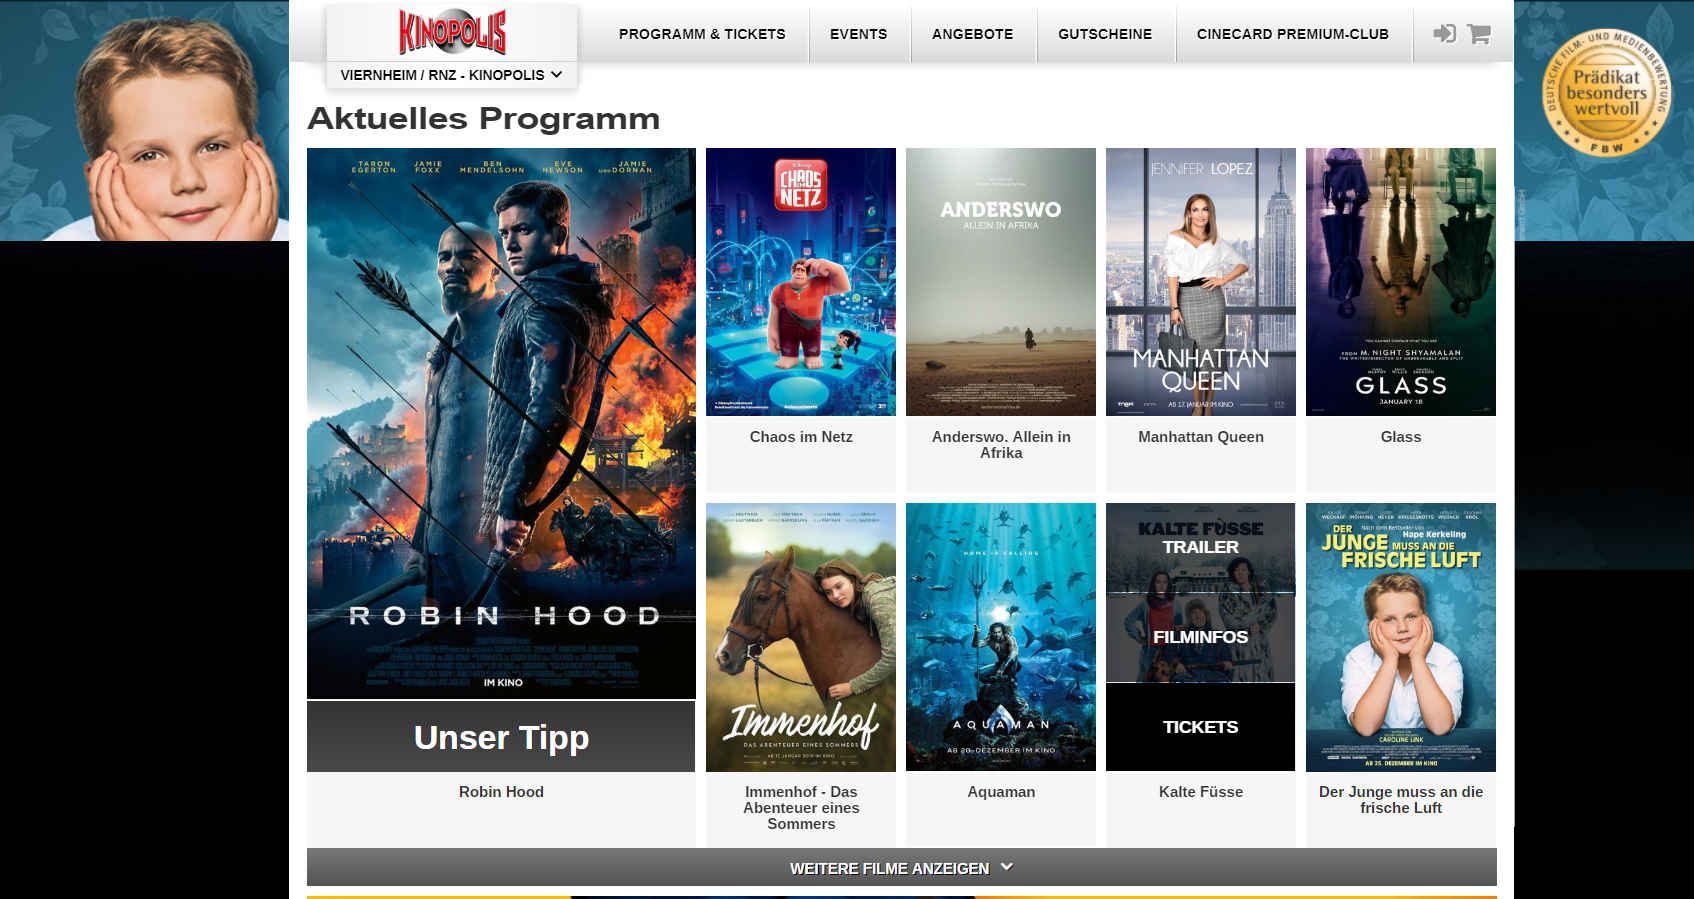
\includegraphics[width=14cm]{img/Kinopolis_MA_Start2.png}
		\captionsetup{format=hang}
		\centering\caption[Startseite von Kinopolis Viernheim]{\label{fig:Kinop.Start2}Startseite \\Quelle: Kinopolis Viernheim}
	\end{figure}
	
	Neben diesen Informationen enthält die Startseite von Kinopolis im unteren Bereich Beschreibungen zu aktuellen Events, wie \enquote{Kids Previews} und \enquote{Ladykino}. Darüber hinaus bieten darunterliegende Abschnitte Auskunft zu Filmen, die in näherer Zukunft anlaufen werden, sowie Nachrichten aus Hollywood. 
	
	\subsubsection{Programm \& Filme}
	Die zweite Möglichkeit zur Auswahl eines Filmes besteht durch die Auswahlmöglichkeit \enquote{Programm \& Tickets} in der Kopfleiste. Dort befindet sich zunächst eine Leiste, in der die Vorstellungen für einen bestimmten Tag oder für eine ganze Woche angezeigt werden können. Standardmäßig ist die Übersicht einer Woche ausgewählt, wodurch zu jedem Film alle Vorstellungen der Woche aufgelistet sind. Neben der zeitlichen Eingrenzung der Suche, können mithilfe des ausgeklappten Programmfilters (siehe Abb. \vref{fig:PuT1}) weitere Eingrenzungen vorgenommen werden. Die Filterung kann nach Genre, FSK-Stufen, Art der Darstellung (2D, 3D,...) und nach zeitlicher Eingrenzung eines Tages erfolgen. Mit der zuletzt genannten Filtermöglichkeit, wird der Zeitpunkt der Vorstellungen in Vormittag, Nachmittag und Abend eingestuft.
	\begin{figure}[H]
		\centering 
		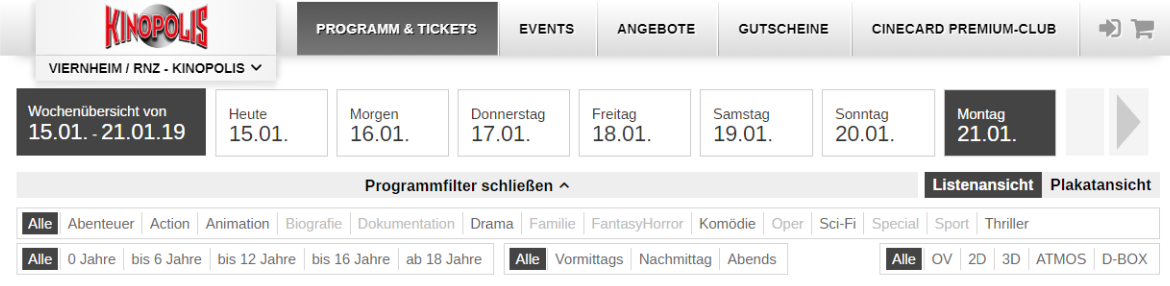
\includegraphics[width=14cm]{img/PuT_1.png}
		\captionsetup{format=hang}
		\centering\caption[Startseite von Kinopolis Viernheim]{\label{fig:PuT1}Programm \& Tickets \\Quelle: Kinopolis Viernheim}
	\end{figure}
	
	Die darunterliegende Darstellung der Filme kann der Nutzer, seiner Präferenz entsprechend, verstellen. Rechts von dem Programmfilter stehen Listenansicht und Plakatansicht zur Auswahl. Voreingestellt ist die Listenansicht, in der die Filme untereinander dargestellt werden. Zu jedem Film sind Eckdaten wie das Genre, die Länge, und das Startdatum angegeben (siehe Abb. \vref{fig:PuT2}). Außerdem wird durch Labels unterstützend ersichtlich, welche FSK-Stufe für den Film besteht. Zusätzliche Labels unterrichten den Nutzer über spezielle Events sowie Angebote. Des Weiteren wird ein Überblick über die Vorstellungen eines Films der kommenden Woche geboten. Dabei wird neben der Zeit ebenfalls der Saal angegeben. 
	\begin{figure}[H]
		\centering 
		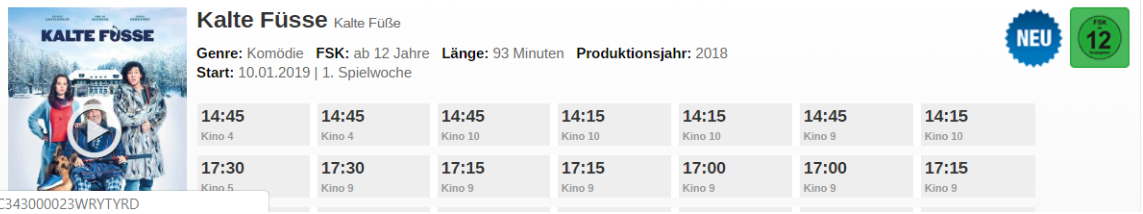
\includegraphics[width=14cm]{img/PuT_2.png}
		\captionsetup{format=hang}
		\centering\caption[Programm \& Tickets]{\label{fig:PuT2}Programm \& Tickets \\Quelle: Kinopolis Viernheim}
	\end{figure}
	
	Durch das Überfahren einer Vorstellung mit der Maus bekommt der Nutzer die Eckdaten des jeweiligen Saals angezeigt (siehe Abb. \vref{fig:PuT3}). Bei speziellen Anforderungen an den Saal kann der Nutzer über den Button \enquote{Saalübersicht} die Daten zu allen vorhandenen Sälen abrufen und somit viel Zeit bei der Suche nach einem Kinosaal sparen, der die Anforderungen erfüllt. Im nächsten Schritt kann der Nutzer entweder weitere Informationen zu einem Film anschauen, indem er auf den Button \enquote{Filminfos} oder auf den Titel klickt. Dadurch wird der Nutzer auf eine Detailseite weitergeleitet, die nachfolgend erläutert wird. Wenn der Nutzer bereits eine Vorstellung ausgewählt hat, wird er durch das Anklicken der Vorstellung auf die Reservierungsseite weitergeleitet. 
	\begin{figure}[H]
		\centering 
		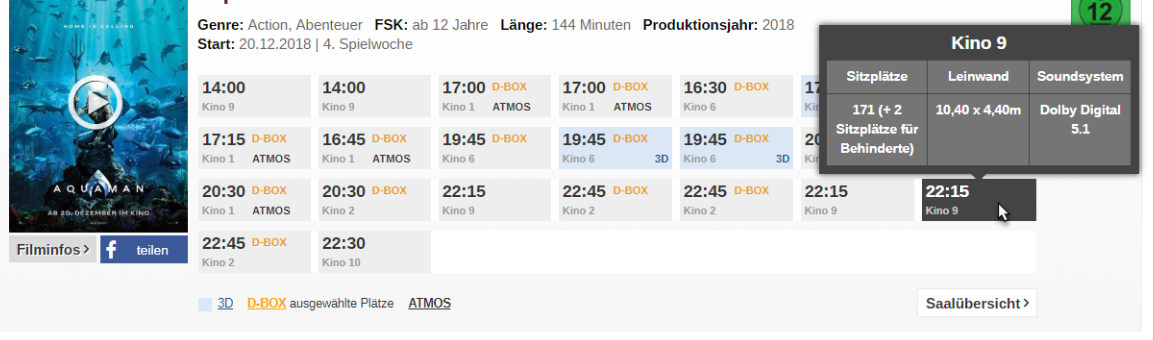
\includegraphics[width=14cm]{img/PuT_3.png}
		\captionsetup{format=hang}
		\centering\caption[Programm \& Tickets]{\label{fig:PuT3}Programm \& Tickets \\Quelle: Kinopolis Viernheim}
	\end{figure}
	
	Die Plakatansicht als zweite Möglichkeit der Darstellung ist ähnlich aufgebaut, wie die Darstellung der Filme auf der Startseite. Der Nutzer sieht die verschiedenen Filmplakate und den Titel dieser. Es liegt also an dem Nutzer, ob er zusätzliche Informationen zu dem Film direkt ersichtlich haben möchte oder nicht.  
	
	Neben den zwei erklärten Seiten, bietet das Portal weitere Seiten mit Informationen über Events, Angebote und anderen Vorteilen, die nicht zwingend zur Reservierung von Karten notwendig sind. Deshalb werden diese Seiten in der Ist-Analyse zwar registriert, aber nicht als essenzielle Anforderungen an ein Kinoreservierungssystem erfasst. Aus diesem Grund werden sie nicht näher erläutert.
	
	\subsubsection{Detailsseite}
	Eine weitere Unterstützung zur Auswahl eines Kinofilms bietet die Detailseite. Sie gibt den Nutzer einen Überblick über einen Film mithilfe des Trailers, den wichtigsten Informationen und den verschiedenen Vorstellungsterminen. Der Nutzer kann diese Seite auf unterschiedlichen Wegen erreichen. In der Startseite erscheint durch das Positionieren der Maus auf dem gewünschten Filmplakat die Option Filminfos (siehe Abb. \vref{fig:Kinop.Start2}). Durch das Anklicken dieser erfolgt die Navigation zur Detailsseite. Ein solcher Button befindet sich ebenfalls in der Seite Programm \& Tickets unterhalb des angezeigten Trailers (siehe Abb. \vref{fig:PuT3}). Zusätzlich enthält sie den Filmtitel, welcher ebenfalls zur Navigation auf die Detailsseite genutzt werden kann. 
	
	Die Detailsseite bietet zunächst eine Auswahl von Videos an. Darunter befindet sich der Trailer und je nach Film weitere Videos, wie das Making-Of. Des Weiteren kann der Nutzer das Filmplakat und eine Bewertung im 5-Sterne-System einsehen und auch selbst abgeben. Nach den Eckdaten des Films gelangt der Nutzer zu einem Bereich, in dem der Inhalt des Film geschildert wird (siehe Abb. \vref{fig:Details}. Dieser ist in deutsch, sowie in einem anderen Tab auch in englisch vorhanden. Ein dritter Tab führt zu Bildern von verschiedenen Szenen des Films. Der darunterliegenden Bereich zeigt eine Übersicht der Vorstellungen in den nächsten sieben Tagen. Jede Vorstellung enthält die Startzeit, den Saal, das Vorhanden sein von speziellen Sitzen und ob der Film in 3D läuft. Als Nächstes wird die Besetzung des Films aufgeführt. Dazu werden die wichtigsten Schauspieler des Films mit ihren Namen und einem Foto gezeigt.
	\begin{figure}[H]
		\centering 
		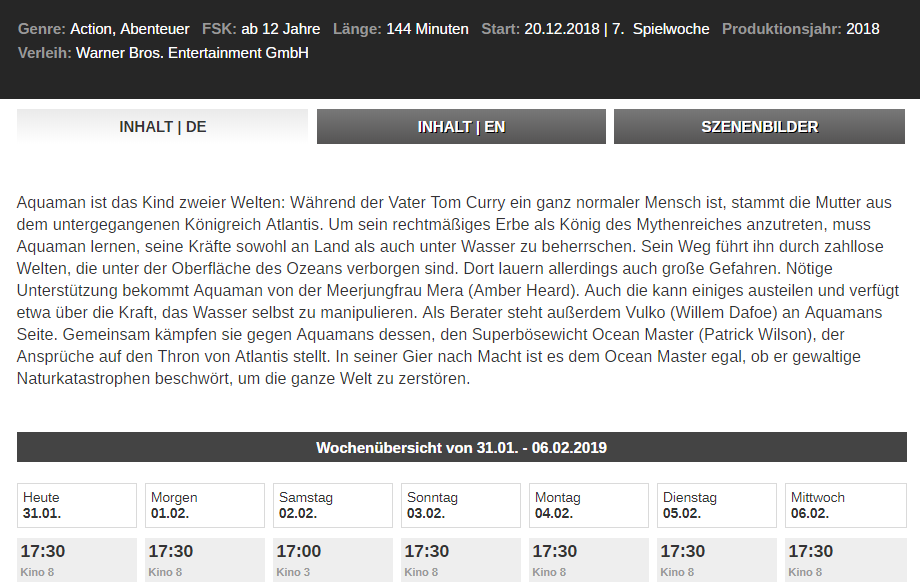
\includegraphics[width=14cm]{img/Detailsseite2.png}
		\captionsetup{format=hang}
		\centering\caption[Startseite von Kinopolis Viernheim]{\label{fig:Details}Detailsseite \\Quelle: Kinopolis Viernheim}
	\end{figure}  
	
	\subsubsection{Reservierungsseite}
	Wenn sich der Nutzer für eine bestimmte Vorstellung eines Films entschieden hat, gelangt er auf verschiedenen Wegen zur Reservierungsseite. Die Auswahl einer Vorstellung kann in der zuletzt vorgestellten Detailseite über die angezeigten Vorstellungen der nächsten Woche erfolgen. Eine weitere Möglichkeit bilden die Seite \enquote{Programm \& Filme} mit ihrer Wochenübersicht der Vorstellungen und die Startseite, in welcher die Navigation durch das Anklicken von \enquote{Tickets} erfolgt. 
	
	Die Reservierungsseite enthält die Möglichkeit in dem Kinosaal der Vorstellung einen Platz auszuwählen. Es wird nochmals das Filmplakat gezeigt, wodurch sich der Nutzer sich sein kann, die Karten für den gewünschten Film auszuwählen. Zusätzlich wird das Datum und die Uhrzeit der Vorstellung angegeben, wodurch eine Verwechslungen verhindert werden.
	
	Nachfolgend kann der Nutzer entscheiden ob er die Karten kaufen oder reservieren möchte, mit dem Unterschied, dass bei einem Kauf der Karten ermäßigte Tickets für Kinder, Schüler, etc. gekauft werden können. Bei einer Reservierung hingegen wird nur die Anzahl der Karten ausgewählt und eventuelle Ermäßigungen werden erst an der Kasse besprochen (siehe Abb. \vref{fig:Reservierung}). Bei dem Vorhandensein von verschiedenen Preiskategorien muss der Kunde zunächst die Kategorie wählen, da in dem nachfolgenden Sitzplan nur Plätze der dazugehörigen Kategorie gewählt werden können. 
	
	Wenn der Nutzer Kategorie und Anzahl der Plätze ausgewählt hat, kann er mithilfe eines visualisierten Sitzplans seine bevorzugten Sitze wählen. Die Darstellung enthält die Position der Leinwand, den Eingang und die Treppen des Saals. Jeder Sitz des Raums ist eingezeichnet und enthält durch seine Darstellung Informationen über den Buchungsstatus. Durch die farblich verschiedenen Plätze kann der Nutzer die Preiskategorien voneinander unterscheiden, sowie auf einen Blick erkennen, welche Plätze bereits belegt oder nicht buchbar sind. 
	
	Hat sich der Nutzer für bestimmte Plätze entschieden, so kann er diese in der Platzkarte auswählen. In diesem Reservierungssystem können nur Plätze nebeneinander gebucht werden, wodurch die gewählte Anzahl der Tickets immer nebeneinander liegen. Nach dem Auswählen verändert sich der Kopf der Seite, sodass der Nutzer die exakten Angaben zu seinen Plätzen bekommt. Beim Kaufvorgang bekommt er zusätzlich detaillierte Angaben zu dem Gesamtpreis. 
	\begin{figure}[H]
		\centering 
		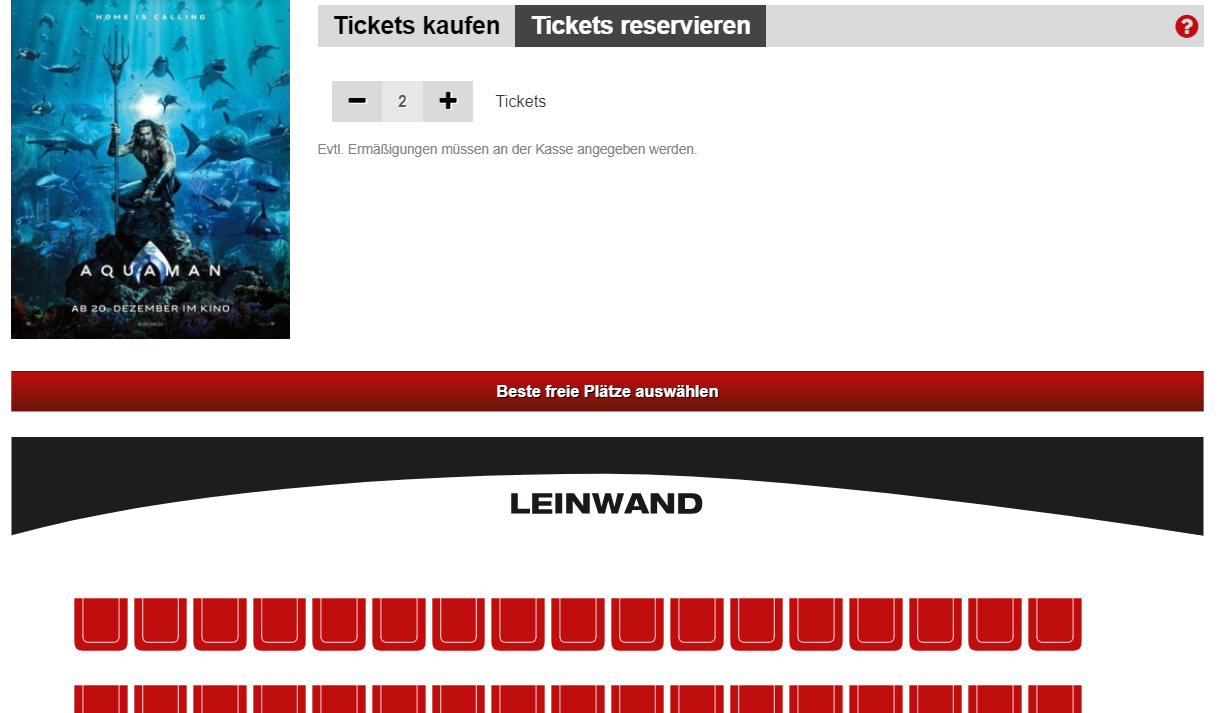
\includegraphics[width=14cm]{img/Reservierungsseite.png}
		\captionsetup{format=hang}
		\centering\caption[Startseite von Kinopolis Viernheim]{\label{fig:Reservierung}Reservierungsseite \\Quelle: Kinopolis Viernheim}
	\end{figure}	
	
	\subsubsection{Warenkorb}
	Über einen Button gelangt der Nutzer zunächst auf eine Seite, die einen Überblick über die gewählten Produkte gibt. Der Nutzer kann sich entscheiden, ob er die Karten mit vorhandenem Kundenkonto über einen Login oder als Gast kaufen bzw. reservieren möchte. Außerdem besteht die Möglichkeit ein neues Nutzerkonto anzulegen. Bei der Wahl des Gastzugangs wird der Nutzer aufgefordert seinen Namen, sowie E-Mail und Geburtsdatum anzugeben. 
	
	Beim Reservieren von Karten können die diese durch den Button \enquote{Jetzt reservieren} reserviert werden, wodurch der Nutzer eine Reservierungsnummer als Bestätigung zugewiesen bekommt (siehe Abb. \vref{fig:Warenkorb}). Mit dieser kann er die Karten bis einer halben Stunde vor Beginn der Vorstellung an der Kasse abholen. Auf der Bestätigungsseite bekommt der Nutzer ebenfalls die Möglichkeit die Reservierung zu drucken, sodass er sie ausgedruckt vorliegen hat. Des Weiteren hat der Kunde die Möglichkeit die Karten zu kaufen oder direkt zu stornieren. 
	\begin{figure}[H]
		\centering 
		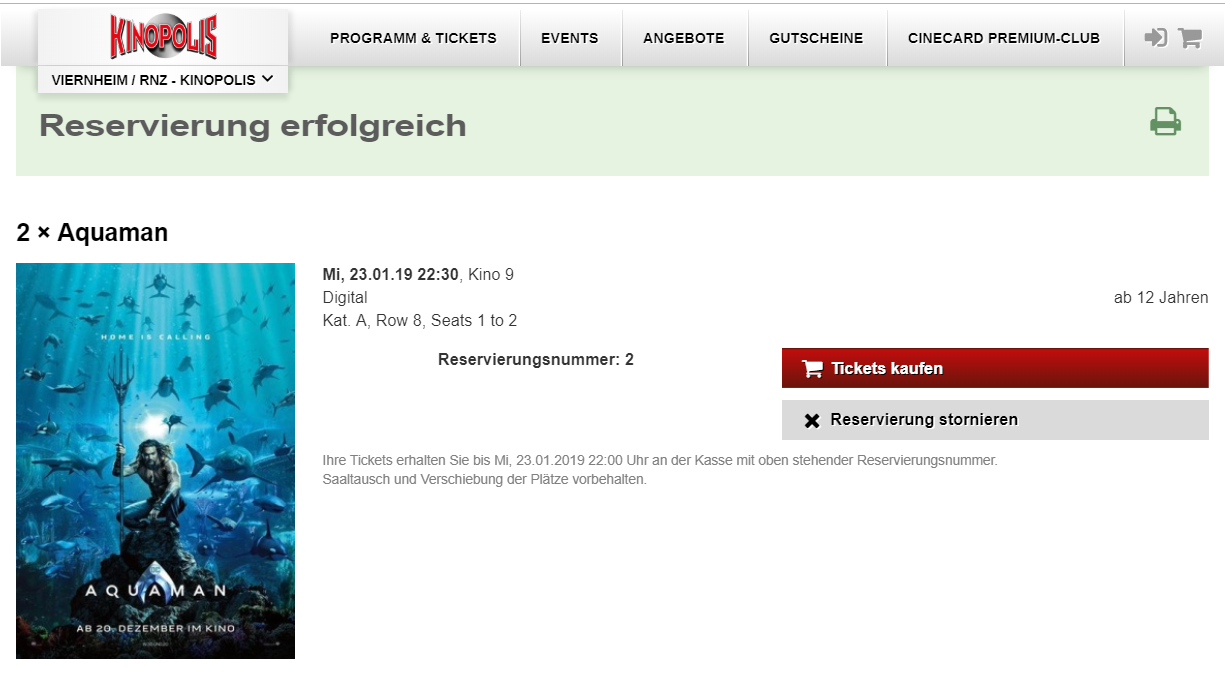
\includegraphics[width=14cm]{img/Warenkorb.png}
		\captionsetup{format=hang}
		\centering\caption[Startseite von Kinopolis Viernheim]{\label{fig:Warenkorb}Warenkorb \\Quelle: Kinopolis Viernheim}
	\end{figure}
	
	In dem Kaufvorgang gelangt der Kunde nach dem Anklicken von \enquote{Weiter} in die Ansicht des Warenkorbs, welche die wichtigsten Informationen zu der Vorstellung und dem Standort des Kinos enthält. Außerdem werden Reihe und Plätze der Sitze mit ihrem dazugehörigen Preis angezeigt. Danach wird die Zahlungsmethode gewählt, wobei die verschiedenen Auswahlmöglichkeiten zunächst schwer zu erkennen sind. Nach der Auswahl werden die Tickets bezahlt und der Kunde kann in dem Kino direkt reingehen ohne sich zuvor an der Kasse anstellen zu müssen. 
	
	\subsubsection{Zusammenfassung der erforderlichen Schritte} 
	Für eine Reservierung von Karten sind vier Schritte von Bedeutung. Zunächst wird der Entscheidungsprozess des Nutzers unterstützt. Dies kann durch den Trailer oder das Lesen der Filmbeschreibung geschehen. Nachfolgend wählt der Kunde einen Tag und eine Uhrzeit aus, an dem er sich den Film anschauen möchte. In dem nächsten Schritt entscheidet er wie viele Plätzen er reservieren bzw. kaufen möchte, sowie wo sich die Sitze in dem Kinosaal befinden sollen. Als letzter Schritt erfolgt die Reservierung der Tickets indem der Kunde seine Daten angibt und dadurch eine Reservierungsnummer mitgeteilt bekommt, mit der er die Karten im Kino abholen kann.
	
	\section[Soll-Analyse]{Soll-Analyse {\hfill \normalsize Milena Zahn}}
		
	 	\subsection{User-Research-Prozess} 
	 	User Research ist eine systematische Untersuchung der Ziele, Bedürfnisse und Fähigkeiten der Benutzer\autocite[Vgl.][S. 6]{Schumacher.2010}.
	 	Durch diesen Prozess lässt sich sicherstellen, dass die entwickelte Software den Nutzern einen Mehrwert bietet und an deren Bedürfnisse angepasst ist.
		Der Prozess startet mit der Identifikation der \textit{User Profiles}. Diese klassifizieren Endanwender mit Nutzerprofilen, damit eine konkrete Vorstellung der Anwender geschaffen wird. Anhand von Beschreibungen von Attributen lässt sich die Nutzergruppe identifizieren.
		
		\begin{table}[H]
			\centering
			\begin{tabular}{p{5,5cm} || c | c }
				\textbf{Attribute} & \textbf{Endanwender} & \textbf{Mitarbeiter} \\\toprule
				Alter &  16 - 99 Jahre &  16 - 99 Jahre \\
				Geschlecht &  männlich und weiblich &  männlich und weiblich  \\
				Medienkompetenz &  ja und nein &  ja  \\
				Erfahrung Onlinereservierung &  ja und nein &  ja  \\
				Anwender &  extern &  intern  \\
			\end{tabular}
			\caption[User Profile]{\label{tab:tabelleUserProfile}User Profile }
		\end{table}
		
		Im nächsten Schritt werden Personas aus den User Profiles erstellt. Personas sind fiktive Personen, die für eine Nutzergruppe steht. Der Zweck von Personas ist, dass Entwickler Empathie und Einfühlungsvermögen zu den konkreten Anwendern aufbauen können. Darüber hinaus bieten den Personas den Vorteil eine Diskussionsgrundlage zu schaffen und damit die Funktionen den Personas angepasst werden. Für das Reservierungs-Tool wurden vier verschiedene Personas, die in Abbildung \vref{fig:personas} dargestellt werden, aus den User Profiles angelegt. 
		
		\begin{figure}[H]
			\subfigure[Persona Franzi]{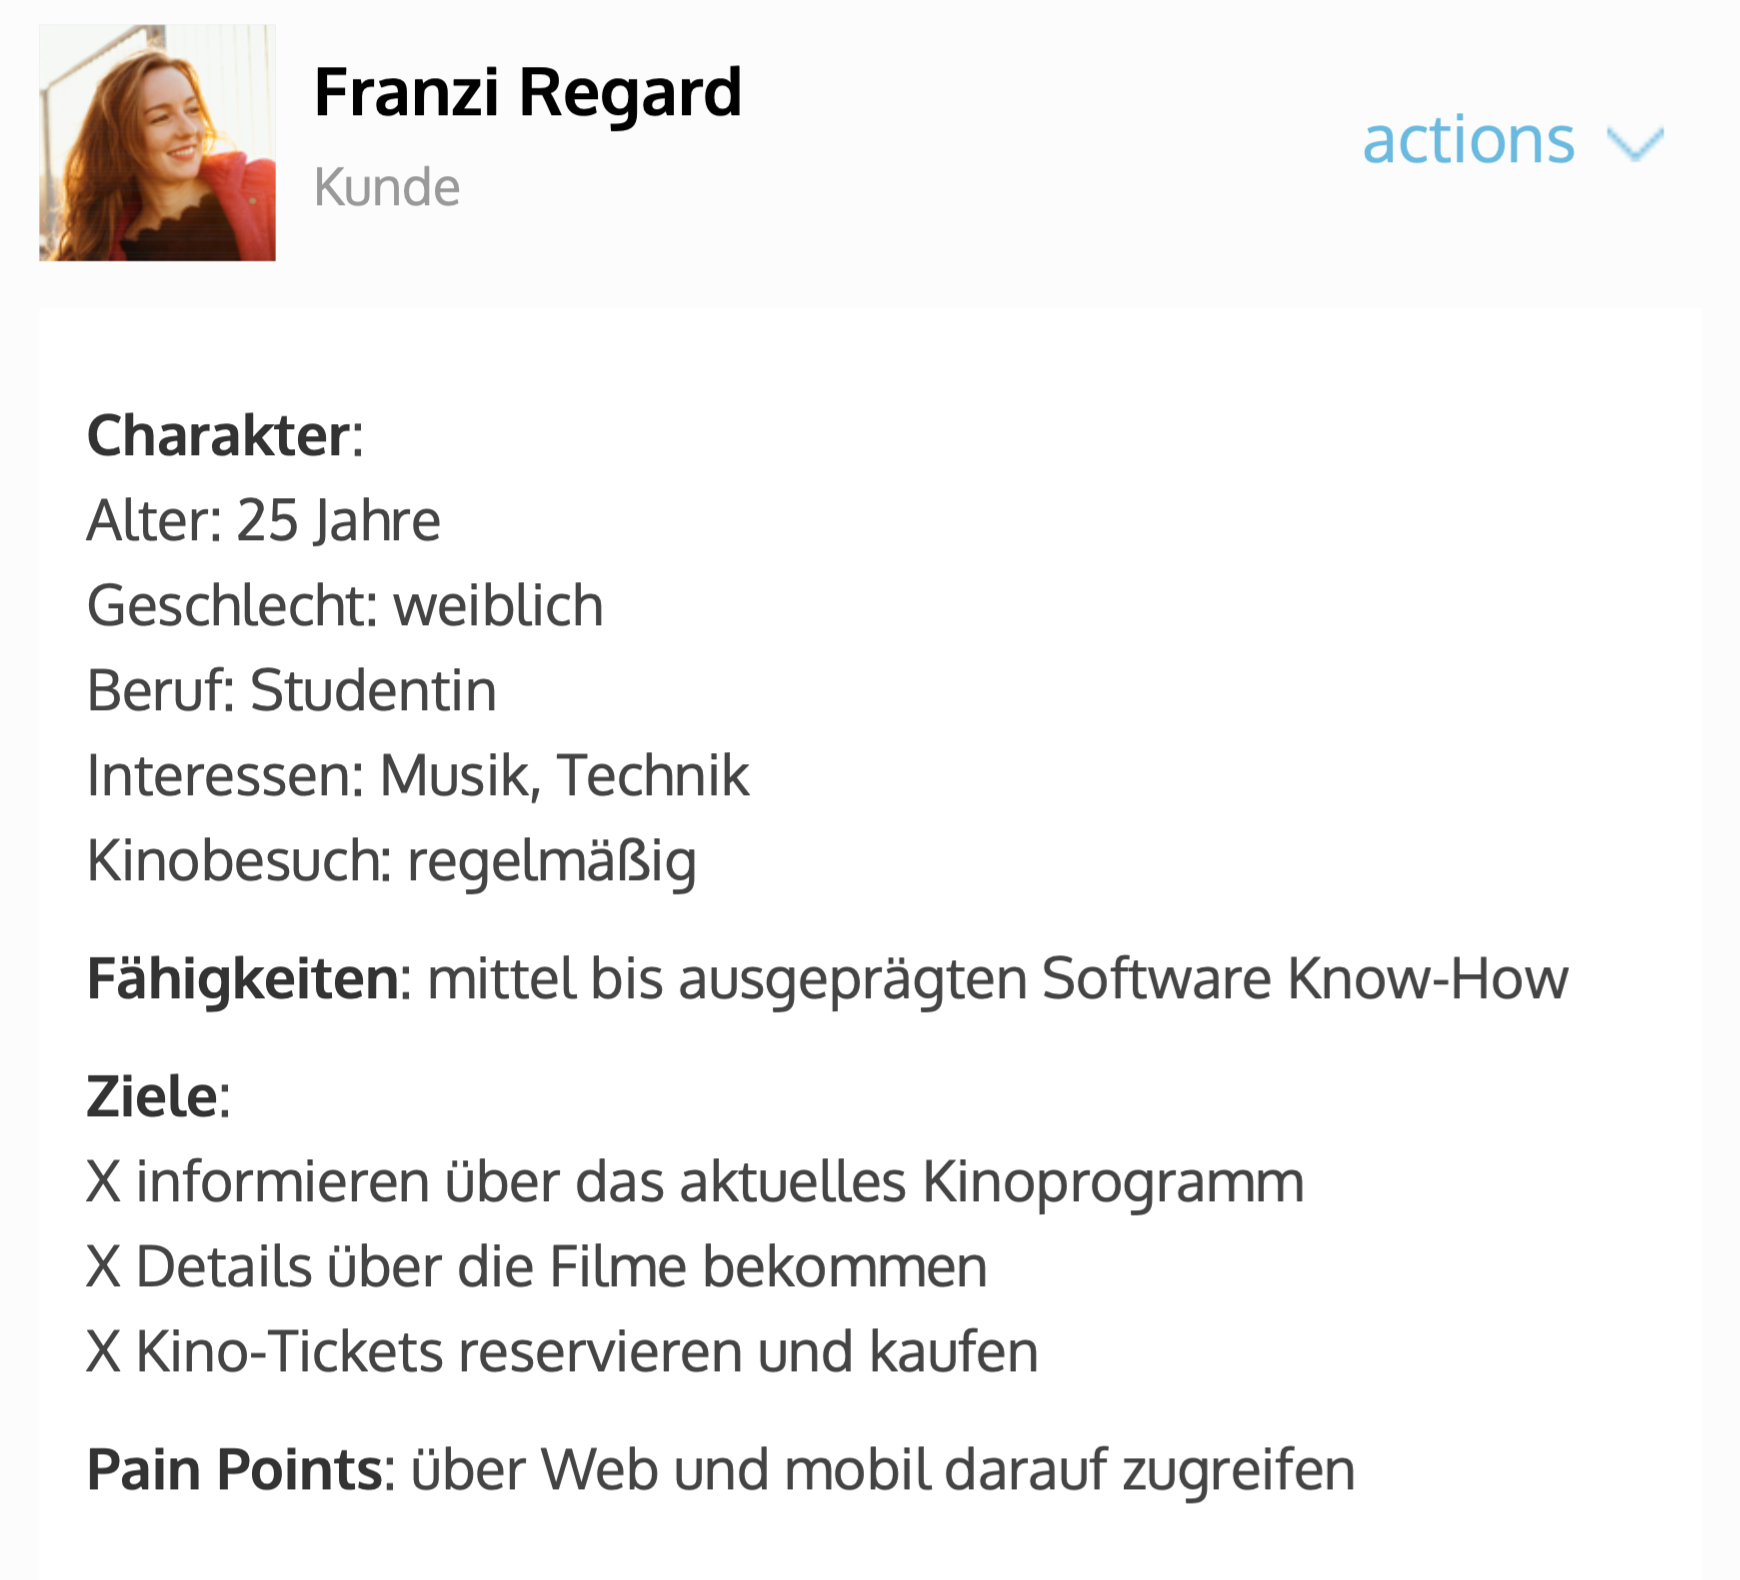
\includegraphics[width=0.49\textwidth]{img/franzi.png}} 
			\subfigure[Persona Gustav]{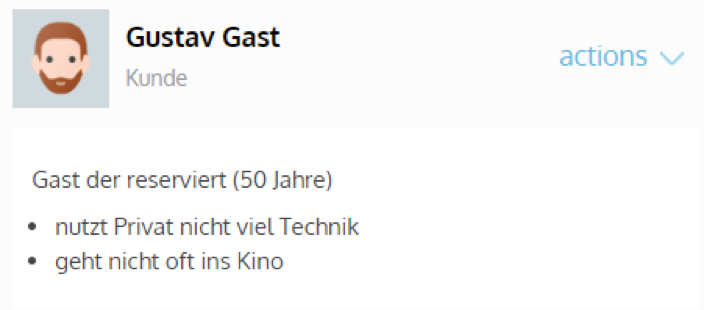
\includegraphics[width=0.49\textwidth]{img/gustav.png}} 
			\subfigure[Persona Kassandra]{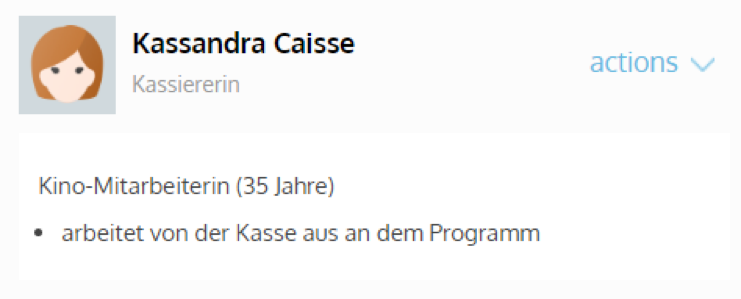
\includegraphics[width=0.49\textwidth]{img/kassandra.png}} 
			\subfigure[Persona Walter]{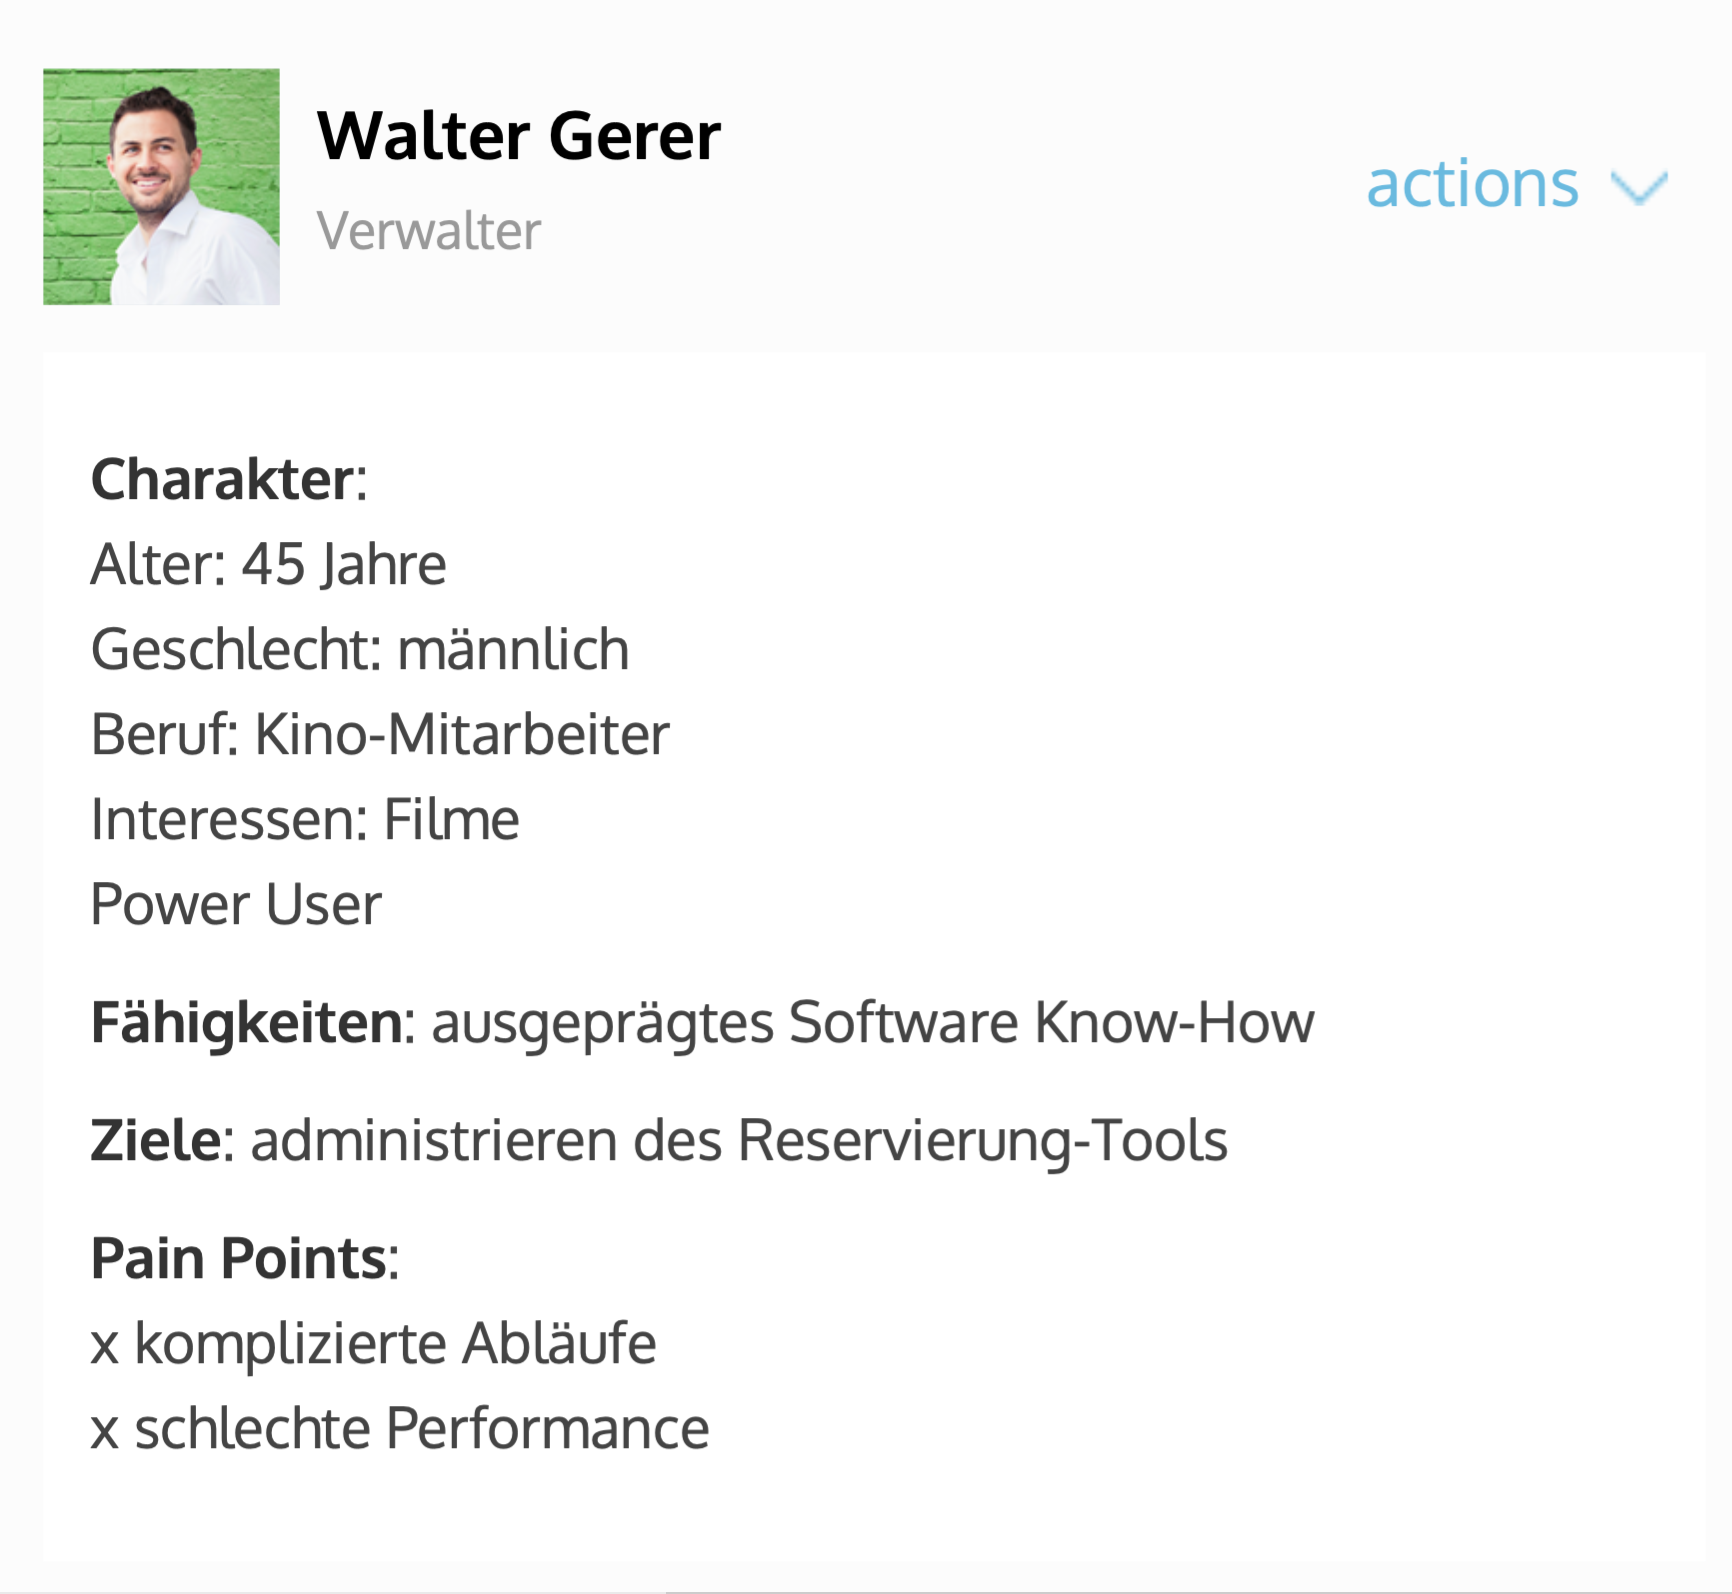
\includegraphics[width=0.49\textwidth]{img/walter.png}} 
			\caption[Personas ]{\label{fig:personas}Personas \\ Quelle: StoriesOnBoard \footnotemark}
		\end{figure} 
		\footnotetext{http://storiesonboard.com}
		
		Darauf aufbauend werden Use Cases für die Personas entwickelt. Diese beschreiben Szenarien, wie die Personas das Endprodukt verwenden werden und welche Vorgehensweisen und Anforderungen sie dabei haben. In den folgenden Abbildungen \ref{fig:useCaseFranzi} bis Abbildung \ref{fig:useCaseWalter2} werden die für die vier Personas erstellten Use Cases dargestellt.
		
		\begin{figure}[H]
			\begin{tabular}{p{13cm}}
				\textbf{Franzi Regard} \\\toprule
				Als Franzi möchte ich Kino-Tickets online reservieren, damit ich mir mit Freunden einen Film im Kino anschauen kann. Dafür möchte ich mich vom meinem Smartphone oder Laptop aus über das aktuelle Kino-Programm informieren. Außerdem möchte ich die Tickets reservieren und dabei angeben, auf welchen genauen Sitzplätzen wir sitzen möchten. Dabei lege ich viel Wert auf ansprechendes Design und Informationen zu den aktuellen Filmen. Um den Besuch so angenehm wie möglich zu haben, möchte ich auch online schon bezahlen können.
			\end{tabular}
			\caption[Use Case Franzi]{\label{fig:useCaseFranzi} Use Case Franzi}
		\end{figure}
	
		\begin{figure}[H]
			\begin{tabular}{p{13cm}}
				\textbf{Franzi Regard} \\\toprule
				Als Franzi möchte ich mir ein Profil erstellen können, damit ich mir meine vorherigen und aktuellen Reservierungen ansehen kann, da ich regelmäßig ins Kino gehe. 
			\end{tabular}
			\caption[Use Case Franzi 2]{\label{fig:useCaseFranzi2} Use Case Franzi 2}
		\end{figure}
	
		\begin{figure}[H]
			\begin{tabular}{p{13cm}}
				\textbf{Gustav Gast} \\\toprule
				Als Gustav möchte ich Kino-Tickets reservieren, um mit meiner Familie einen schönen Familienabend zu verbringen. Eine intuitive Anwendung ist für mich sehr wichtig, weil noch nie online Tickets reserviert habe. Ich möchte auch eine Absicherung bekommen, dass der Vorgang funktioniert hat, da ich sehr unsicher bin mit einer Online-Reservierung.
			\end{tabular}
			\caption[Use Case Gustav]{\label{fig:useCaseGustav} Use Case Gustav}
		\end{figure}
	
		\begin{figure}[H]
			\begin{tabular}{p{13cm}}
				\textbf{Kassandra Caisse} \\\toprule
				Als Kassandra möchte ich mir die aktuellen Reservierungen anschauen und anpassen können. Wenn ein Kunde anruft und seine Reservierung stonieren möchte muss ich darauf reagieren können. Die reservierten Sitze möchte ich auch ändern können und manuell Plätze reservieren.
			\end{tabular}
			\caption[Use Case Kassandra]{\label{fig:useCaseKassandra} Use Case Kassandra}
		\end{figure}

		\begin{figure}[H]
			\begin{tabular}{p{13cm}}
				\textbf{Walter Gerer} \\\toprule
				Als Walter möchte ich das Kino-Programm verwalten. Dafür muss ich neue Filme anlegen und löschen können. Dazu muss ich jeweilis Vorstellungen erstellen, ändern und löschen können. 
			\end{tabular}
			\caption[Use Case Walter]{\label{fig:useCaseWalter} Use Case Walter}
		\end{figure}
	
		\begin{figure}[H]
			\begin{tabular}{p{13cm}}
				\textbf{Walter Gerer} \\\toprule
				Als Walter möchte die Kunden- und Mitarbeiterkonten bearbeiten können, damit ich diese verwalten kann. Dazu muss ich jeweilis Konten erstellen, ändern und löschen können. 
			\end{tabular}
			\caption[Use Case Walter 2]{\label{fig:useCaseWalter2} Use Case Walter 2}
		\end{figure}
		
	\subsection{User-Story-Mapping}
	Schließlich wird aus den Personas und den Use Cases das User-Story-Mapping erstellt. Das User-Story-Mapping ist \enquote{eine schlanke und sehr effiziente Methode} \autocite[][S. 143]{userStory}, um die die Reihenfolge der Anforderungen, die realisiert werden sollen, zu koordinieren. In dieser werden die aus den Use-Cases hervorgehenden Features visuell geplant und in unterschiedliche Releases priorisiert. Dafür wurde das Online-Tool \enquote{StoriesOnBoard}\footnote{https://storiesonboard.com} genutzt. In dieser Software konnten ebenfalls die Personas angelegt werden, damit diese den Aktivitäten zugeordnet werden können. In Abbildung \vref{fig:userStoryMap} ist die erstellte User-Story-Map dargestellt. In Abbildung \ref{fig:userStoryMap}(a) sieht man den ersten Teil, wobei der Teil 2 in Abbildung \ref{fig:userStoryMap}(b) in der Online-Software direkt nebenan dargestellt wird. 
	
	Der erste Schritt ist die Ermittlung der Projektziele. Es werden die Ziele der Personas die aus den Use Cases hervorgehen zusammengefasst. Diese werden auf den blauen Karteikarten aufgelistet und in eine logische Reihenfolge gebracht. Den Zielen werden die entsprechenden Personas zugeordnet (in den Abbildungen leider nicht wie in dem Online-Tool erkennbar). Nachdem die Ziele gesammelt wurden, werden die einzelnen Benutzerschritte auf den darunter liegenden gelben Karteikarten festgehalten. Man identifiziert die Schritte, die der Benutzer unternimmt bzw. durchläuft, um sein Ziel zu erreichen. Der dritte Schritt ist es Lösungsmöglichkeiten und erforderliche Funktionen, also die User-Stories, auf die weißen Karteikarten zu schreiben. Nach diesem Brainstorming-Prozess sind nun alle Ideen festgehalten. Die User Stories haben unterschiedliche Prioritätsstufen und werden in Releases unterteilt. Nach dem häufigsten Verhalten und der grundlegenden Lösung des Reservierungs-Tool wurden die User-Stories priorisiert und das \enquote{Walking Skeleton} erstellt. 
	
	 Die Abbildung \ref{fig:userStoryMap}(a) stellt die wichtigsten Ziele des Prototypen dar. Zum einen ist dies eine Übersicht der aktuellen Filme. Dabei sollen die Kunden einen Überblick über das Kino-Programm bekommen und erste Informationen zu den Vorstellungen. Zum anderen soll ein Benutzer Sitze reservieren können. Dafür muss er zunächst einen Film, Datum und Uhrzeit auswählen. Danach kann er die Sitzplätze zu der Vorstellung aussuchen. Der Reservierungsprozess war zunächst nur für Benutzer mit Kundenkonto vorgesehen, wodurch der Endnutzer die Schritte Login oder Regestrieren durchläuft. Als Bestätigung soll der Nutzer die Bestellnummer bekommen. 
	 
	 Abbildung \ref{fig:userStoryMap}(b) zeigt die weiteren geplanten Funktionen bezüglich dem \enquote{Kundenkonto}. Die administrativen Ziele, die die Use Cases \ref{fig:useCaseKassandra} bis \ref{fig:useCaseWalter2} beschreiben, wurden in das zweite Release eingestuft, da diese nicht zu dem \enquote{Minimum Viable Product} gehören. Im Rahmen des Projektes ist die Umsetzung des Walking Skeleton geplant und das zweite Release, aufgrund der beschränkten Zeit, für die weitere Umsetzung nach dem Projekt geplant.

	\begin{figure}[H]
		\subfigure[Teil 1]{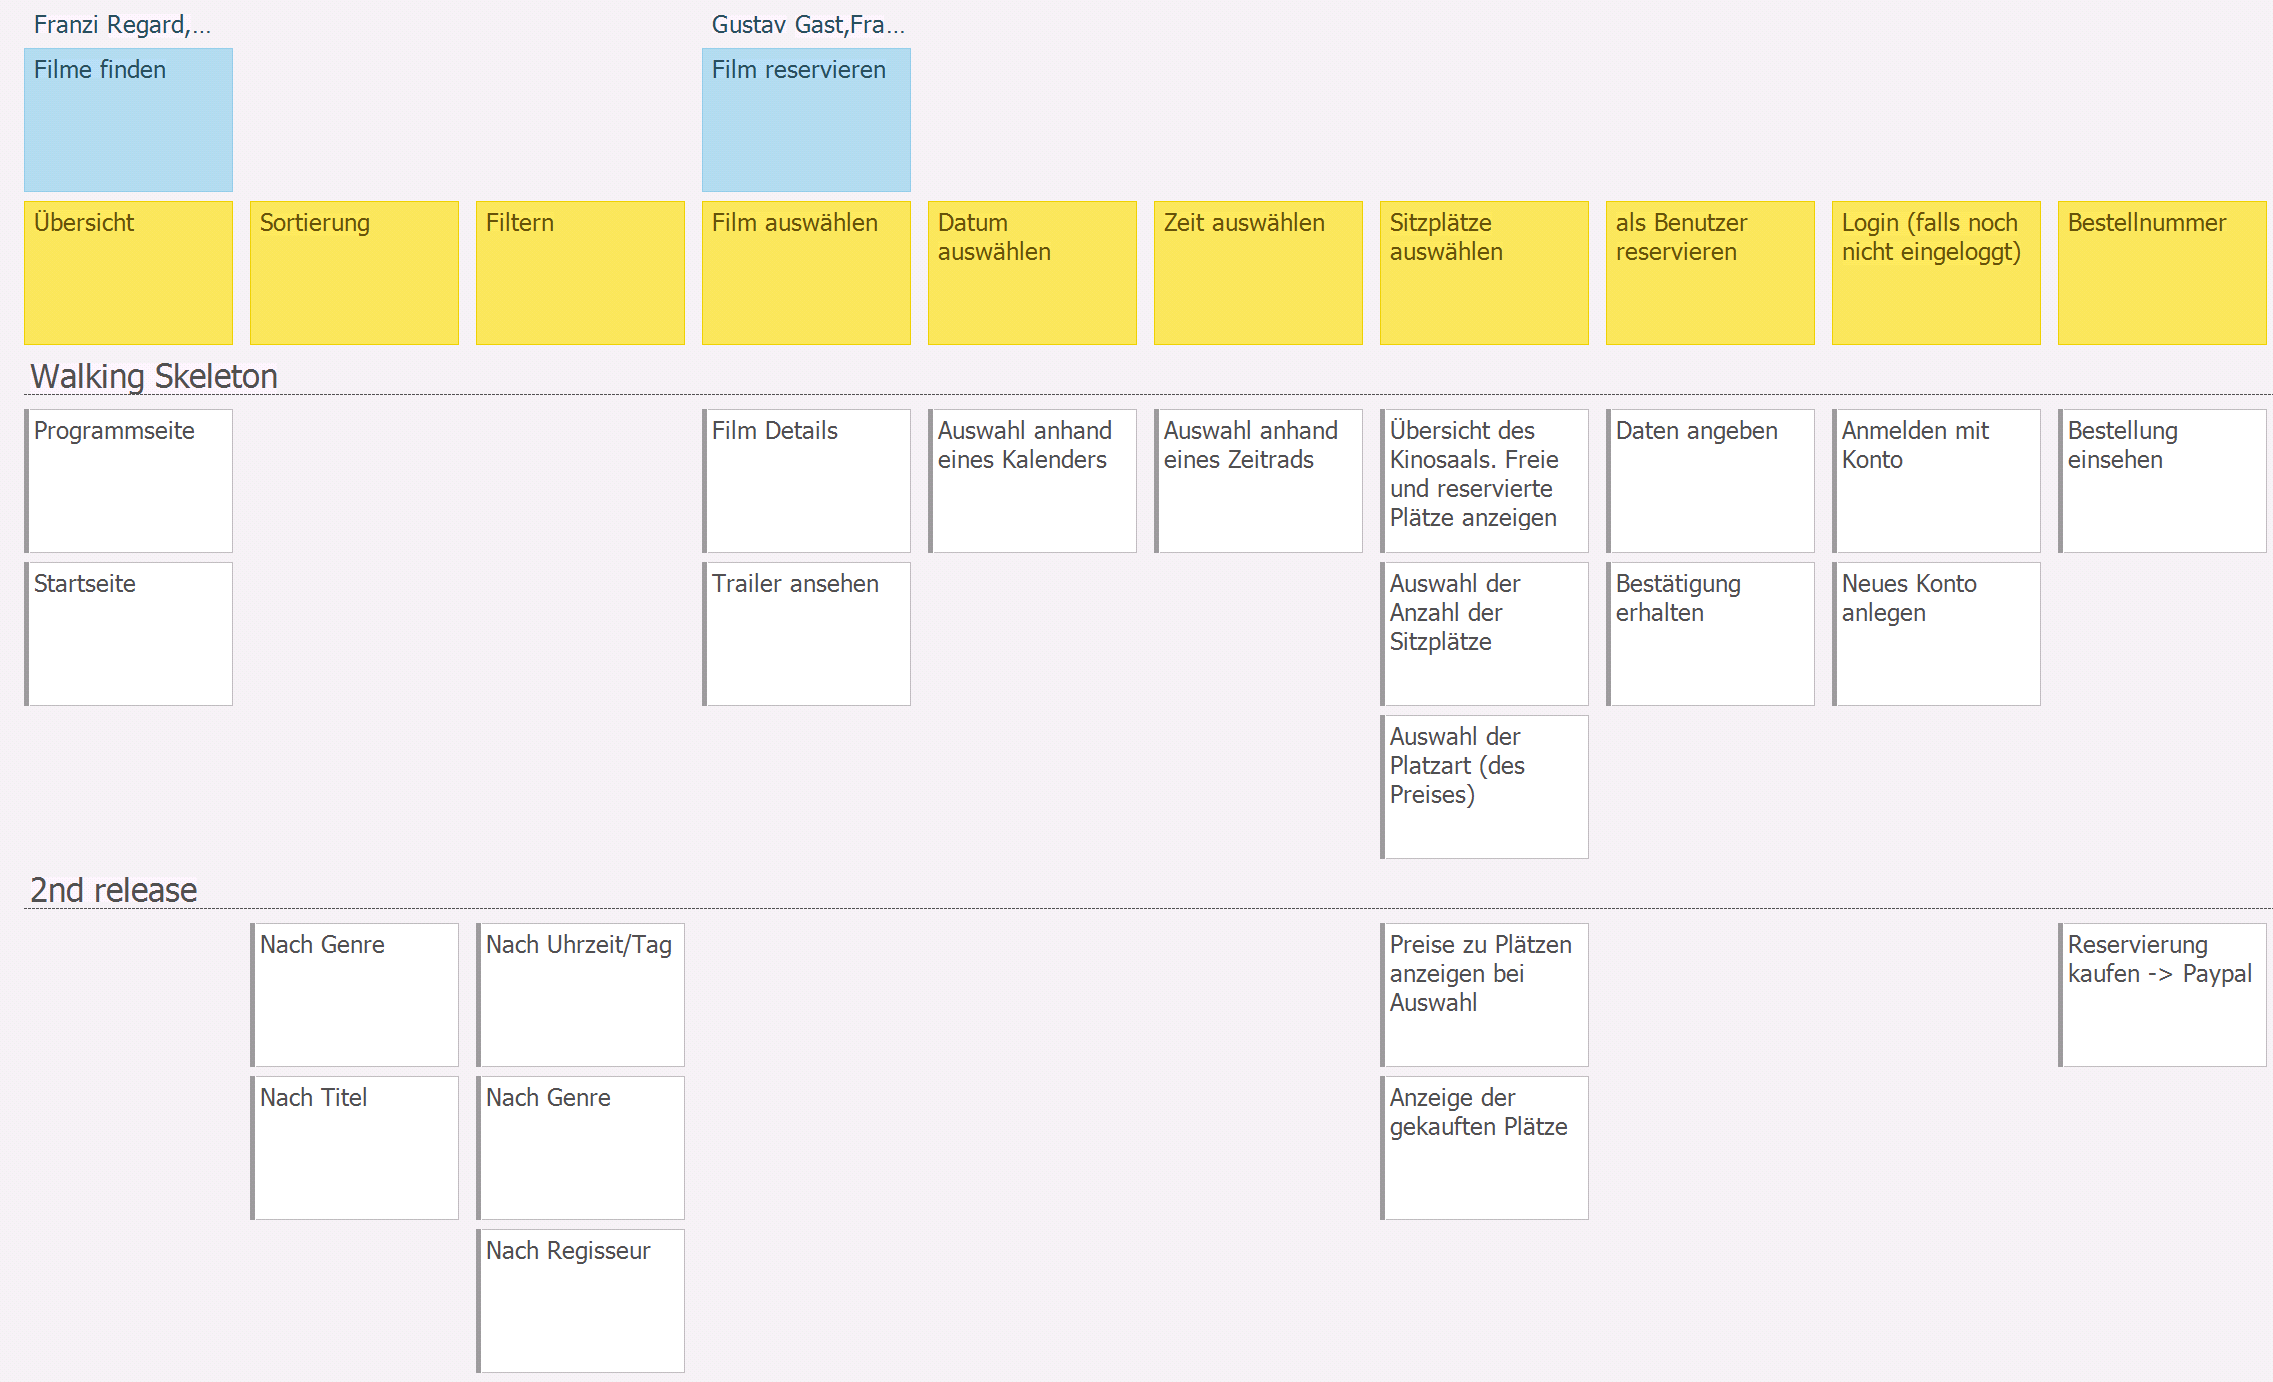
\includegraphics[width=14cm]{img/usm1.png}} 
		\subfigure[Teil 2]{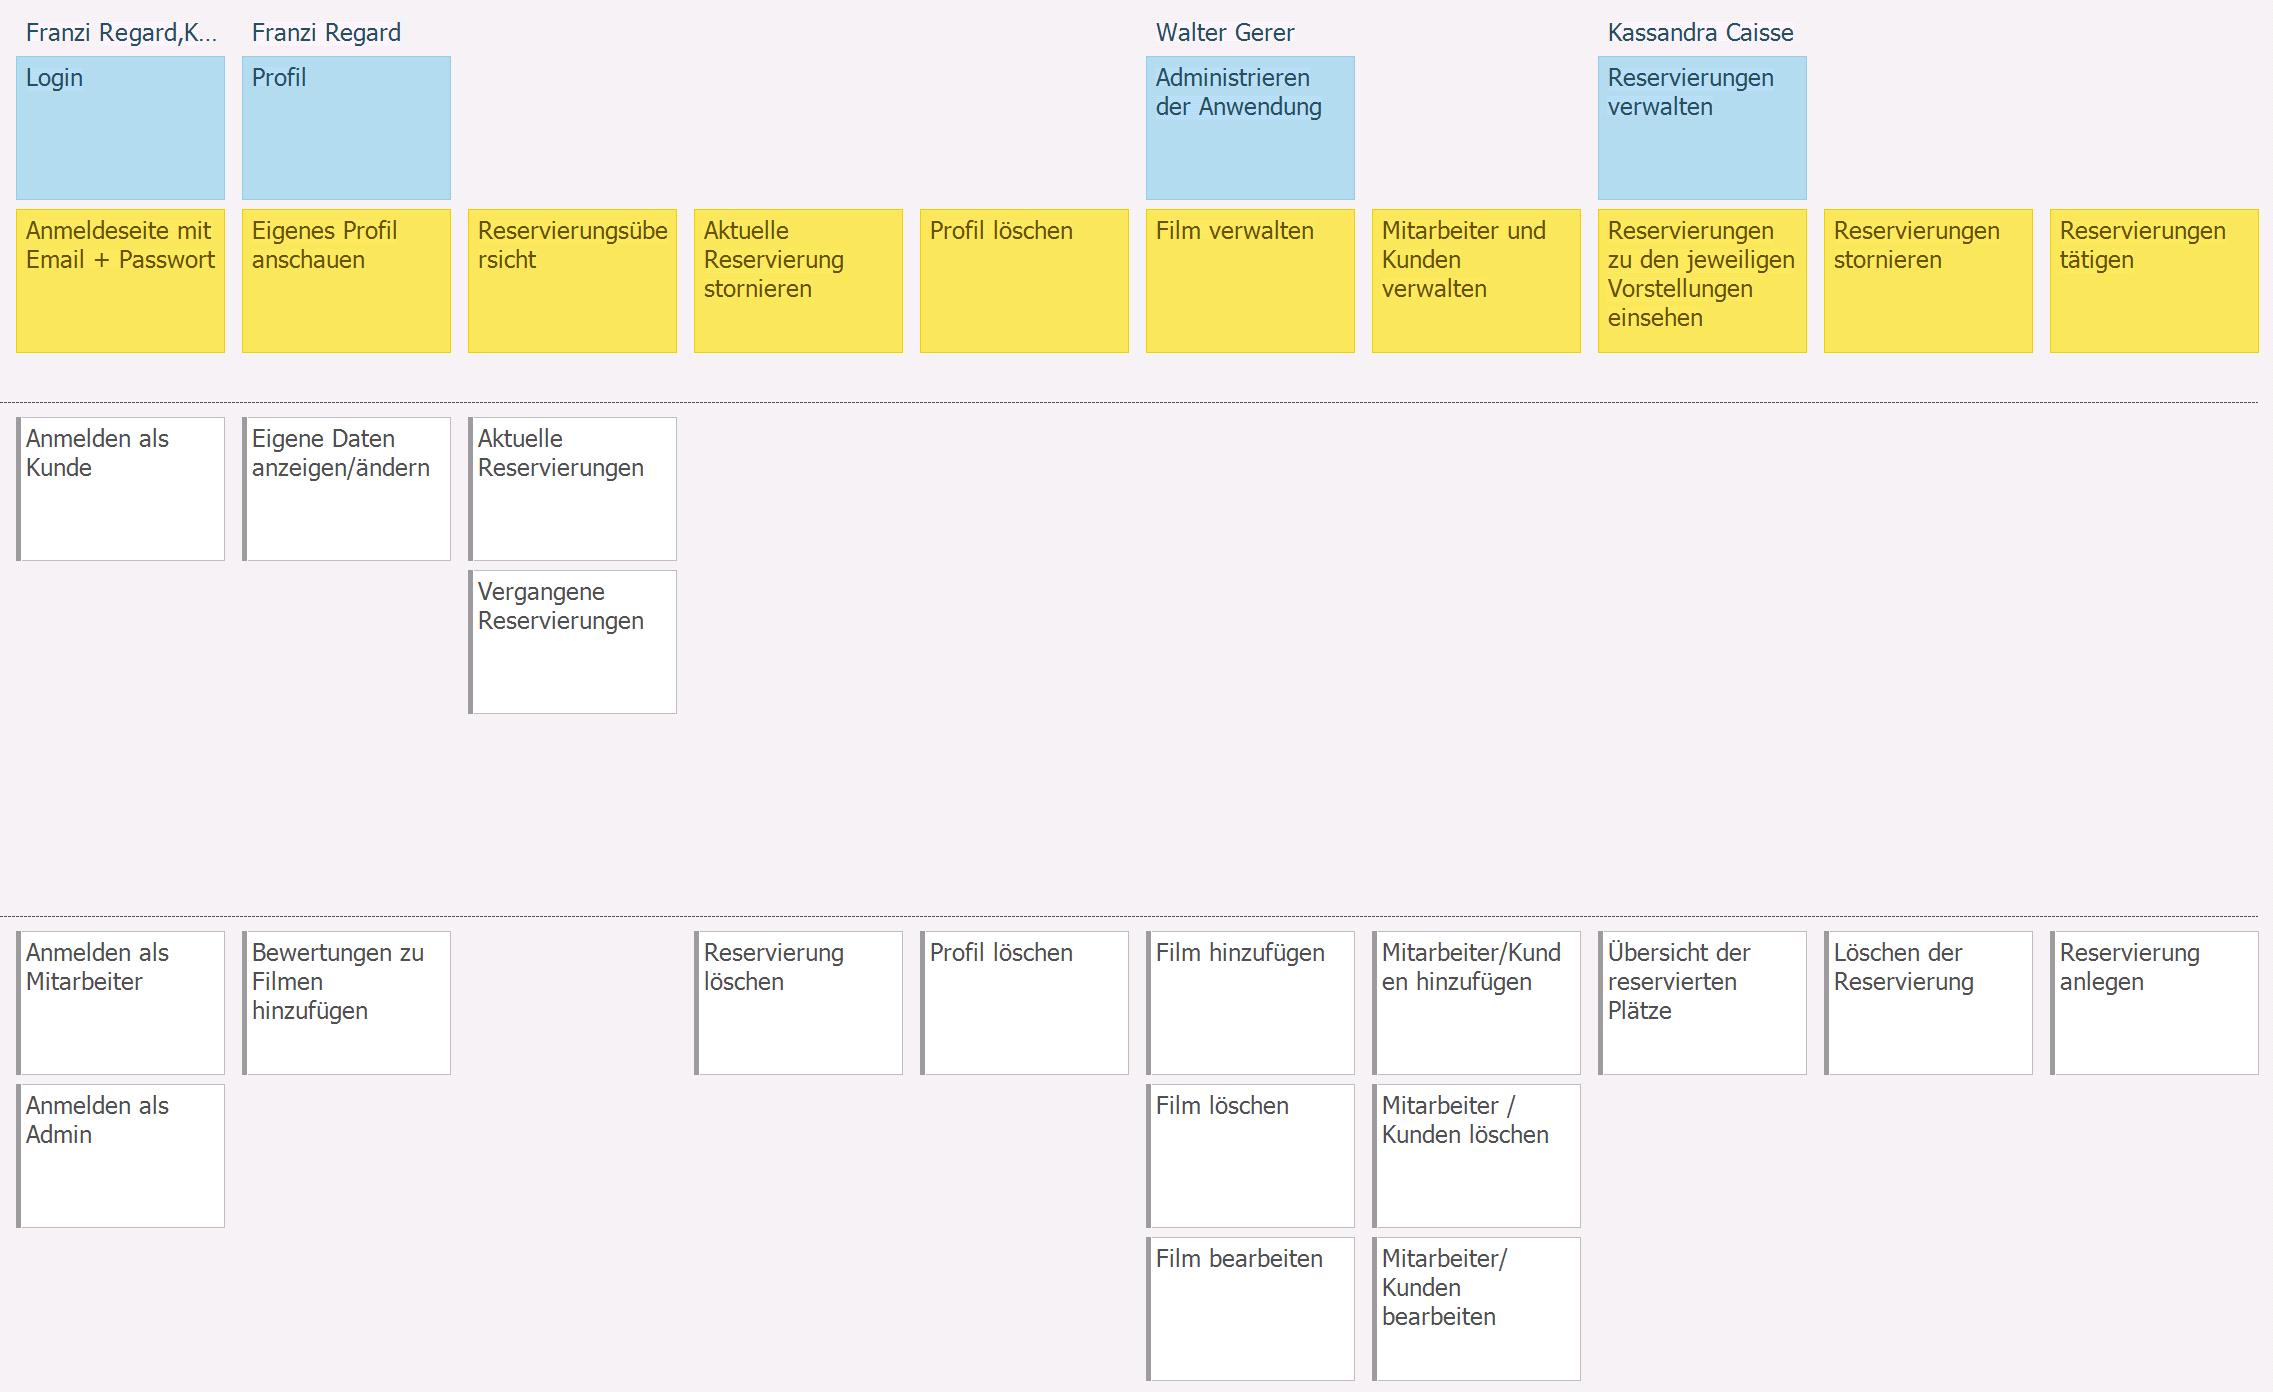
\includegraphics[width=14cm]{img/usm2.png}} 
		\caption[User-Story-Map ]{\label{fig:userStoryMap}User-Story-Map\\ Quelle: Stories on Board}
	\end{figure} 
	 	
%		\subsection{Vorgabe}
%		\subsection{Rahmenbedingungen}
%		\subsection{Bewertungskriterien}